\chapter{Mock Data Challenge}
\label{chap:MDC}

To validate the method developed in this thesis, we conduct a \acf{MDC} using simulated \ac{GW} events and a mock galaxy catalog. The goal of this challenge is to assess the robustness of our inference pipelines and the impact of different brightness cuts on the measurements derived from \ac{GW} observations. The \ac{MDC} is designed to mimic real-world scenarios, allowing us to evaluate the performance of our methods under controlled conditions. This is done with the help of the \texttt{BUZZARD} mock catalogs, which provide a realistic simulation of the galaxy distribution and properties in the universe. 

The \ac{MDC} will involve generating synthetic \ac{GW} events, simulating their detection by the \acf{LVK} detectors, and analyzing the resulting data using the \texttt{gwcosmo} inference pipelines. It is designed to determine the optimal brightness threshold which maximizes the measurement precision with bright subsets while keeping the biases in control. Tests performed in the process will help refine the methodology and ensure that the improved constraints on the Hubble constant are robust against additional systematic uncertainties.

\section{The \texttt{BUZZARD} Mock Catalog}
Cosmological analyses increasingly rely on simulated galaxy catalogs to test, validate, and calibrate inference pipelines. Among the most sophisticated of these are the \texttt{BUZZARD} mock catalogs presented by \citet{DES:2019jmj}, a suite of synthetic sky simulations designed to closely emulate observations from the \acf{DES}. The \texttt{BUZZARD} project aims to produce realistic mock universes that replicate the key statistical, spatial, and photometric properties of large-area surveys~\citep{DES:2019jmj,DES:2021bwg}. These mocks are particularly useful for evaluating systematic uncertainties, testing survey strategies, and validating cosmological pipelines, including those involving standard sirens.

The \texttt{BUZZARD} mocks are constructed through a multi-step process that integrates large-scale dark matter simulations with empirical galaxy assignment and ray-traced gravitational lensing. The underlying dark matter distribution is generated using $N$-body simulations run using the 2LPT{\small{IC}}~\citep{crocce2006transients} and LGADGET2 code~\citep{springel2005cosmological}. The simulations follow the evolution of particles under gravity across large comoving volumes, capturing the hierarchical growth of structure in a flat $\Lambda$CDM cosmology. The cosmological parameters used in the simulation are detailed in Table~\ref{tab:BUZZARD_cosmology}. Three lightcones covering different redshift regimes, denoted L1, L2, and L3, are used to build a deep mock catalog that spans from redshift $z \sim 0$ to $z \sim 2.35$, with increasing resolution and particle number at lower redshifts to mimic the increasing survey completeness at low $z$.

\begin{table}
    \small
    \centering
    \caption[\texttt{BUZZARD} cosmology]{The $\Lambda$CDM cosmology parameters used in the \texttt{BUZZARD} simulations.}
    \label{tab:BUZZARD_cosmology}
    \begin{tabular}{l l c}
        \hline
        \textbf{Parameter} & \textbf{Description} & \textbf{Value} \\
        \hline
        $\Omega_m$ & Matter density parameter & $0.286$ \\
        $H_0$ & Hubble constant & $70~{\mathrm{km}~\mathrm{s}^{-1}~\mathrm{Mpc}^{-1}}$ \\
        $\sigma_8$ & Matter density fluctuation quantifying the   & \\
        & clumpiness of matter distribution & $0.815$ \\
        $n_s$ & Scalar spectral index: scale dependence & \\
        & of the primordial density perturbations & $0.965$ \\
        $\Omega_b$ & Baryon density parameter & $0.046$ \\
        $N_{\mathrm{eff}}$ & Effective number of neutrino species & $3.046$ \\
        \hline
    \end{tabular}
\end{table}

Dark matter halos are identified in the simulation snapshots using the ROCKSTAR halo finder~\citep{behroozi2012rockstar}, which groups particles into gravitationally bound objects based on adaptive phase-space density estimation. Temporal halo merger trees are constructed with the CONSISTENT-TREES algorithm~\citep{behroozi2012gravitationally}, enabling tracking of individual halos across cosmic time. These trees are crucial for assigning realistic galaxy properties and modeling assembly history.

Once the halo population is established, galaxies are inserted using the \ac{ADDGALS} algorithm~\citep{wechsler2022addgals}. \ac{ADDGALS} is a semi-empirical prescription that associates galaxies with dark matter particles based on the local density field, using relationships inferred from observations such as the \ac{SDSS}. Specifically, the algorithm calibrates the conditional luminosity function, the probability of a galaxy having a given luminosity in a particular local density environment, such that the final galaxy sample reproduces the observed luminosity function and galaxy clustering statistics~\citep{DES:2019jmj,wechsler2022addgals}.

Each synthetic galaxy is assigned rest-frame and observed-frame photometry in multiple \ac{DES} bands (e.g., $g$, $r$, $i$, $z$), drawn from a training set derived from real \ac{SDSS} data~\citep{DES:2019jmj}. This ensures that the color-magnitude distribution of \texttt{BUZZARD} galaxies matches the data, which is essential for generating realistic photometric redshifts. Photometric errors and selection effects are modeled to mimic \ac{DES} observations, including depth variations and photometric scatter.

An important feature of \texttt{BUZZARD} is the inclusion of weak gravitational lensing through full-sky ray-tracing with the CALCLENS algorithm~\citep{becker2013calclens}. CALCLENS computes the lensing convergence, shear, and magnification along each line of sight by integrating over the matter distribution in the simulation. These quantities are then assigned to each galaxy, enabling synthetic lensing measurements. This is particularly important for cosmological studies involving large-scale structure, cosmic shear, and galaxy bias calibration.

The final \texttt{BUZZARD} realizations contain over 800 million galaxies each and cover more than 10,000 square degrees of sky, comparable to the footprint of the full \ac{DES}. The mocks include a variety of galaxy samples such as REDMAGIC (a luminous red galaxy sample with low photo-z scatter) and METACALIBRATION (used for weak lensing shear measurements). These samples are used in key \ac{DES} analyses and their inclusion in \texttt{BUZZARD} makes the mock catalogs highly relevant for pipeline validation.

\texttt{BUZZARD} has been extensively validated against \ac{DES} Year 1 (Y1)--\ac{DES} Year 3 (Y3) data, demonstrating good agreement in angular correlation functions, redshift distributions, galaxy-galaxy lensing signals, and shear measurements. The photometric redshift performance in \texttt{BUZZARD} mimics that of \ac{DES} pipelines, allowing realistic estimation of redshift uncertainty impacts~\citep{DES:2019jmj,DES:2021bwg}. These qualities make \texttt{BUZZARD} an ideal environment for end-to-end tests of cosmological inference workflows.

The first \texttt{BUZZARD} data release, \texttt{BUZZARD} DR1, has been made publicly available. It consists of multiple simulations to generate a mock galaxy catalog covering the same sky area as the \acf{DES} surveys. It contains more than 3 billion galaxies with realistic properties, including redshift distributions, luminosity functions, and clustering statistics. In order to facilitate simulated analyses of existing and upcoming large scale structure surveys, photometry is provided in multiple bands, including the DECam ($u,g,r,i,z,Y$), VISTA ($z,Y,J,H,Ks$), WISE ($W1,W2$), Rubin ($u,g,r,i,z,Y$), and Roman ($Y,J,H,K$) passbands.

In this thesis, the \texttt{BUZZARD} mock catalog is used to evaluate the impact of galaxy catalog properties on the measurement of the Hubble constant $H_0$ from dark sirens. Specifically, they allow controlled tests of how catalog pruning, for instance, selecting only the brightest galaxies, affects the redshift prior and the resulting cosmological inference. Because \texttt{BUZZARD} includes realistic magnitude distributions, redshift evolution, and clustering properties, it provides a physically motivated and statistically robust testbed for these experiments.

For our analysis, we use the Roman $K$-band luminosities of the galaxies in the \texttt{BUZZARD} catalog, based on the rationale that $K$-band luminosities are good tracers for the stellar mass~\citep{strazzullo2006near,sureshkumar2021galaxy}. Furthermore, we apply an apparent magnitude threshold of 18 to the catalog to replicate realistic observational conditions, albeit with a somewhat optimistic depth. This apparent magnitude cut is chosen to ensure that the catalog contains a sufficient number of galaxies for statistical analysis. The resulting catalog, referred to as \texttt{BUZZARDm18}, contains approximately 9.2 million galaxies with $K$-band apparent magnitudes brighter than 18, spanning redshifts from $z=0$ to $z=2.35$. The \texttt{BUZZARDm18} catalog, alongside the \ac{GW} events generated by \texttt{GWSim}, detailed in the next section, form a realistic dataset for our analysis. We then use this apparent magnitude limited catalog to select only the brightest galaxies, in order to test our results from \texttt{GLADE+}.

The use of \texttt{BUZZARD} thus supports one of the main goals of this thesis: to develop and validate a method for extracting cosmological information from gravitational-wave observations without electromagnetic counterparts, using only statistically constructed galaxy redshift priors. By using \texttt{BUZZARD} to test this methodology on a simulated sky, we can quantify biases, evaluate uncertainties, and refine our technique.

\section{\texttt{GWSim}}
To validate our methodology and assess the performance of standard siren inference using galaxy catalogs, we require a controlled and physically motivated sample of \ac{GW} events with known properties. For this purpose, we use \texttt{\texttt{GWSim}}~\citep{karathanasis2023gwsim}, a~publicly available Python package designed to generate mock catalogs of \ac{GW} events from \ac{BBH} mergers, incorporating both astrophysical source population models and cosmological assumptions.

\texttt{\texttt{GWSim}} enables simulation of \ac{GW} events from a wide range of mass, spin, and merger rate distributions, within cosmological frameworks such as flat $\Lambda$CDM, $w_0$CDM, and $w_0\text{--}w_a$CDM models. Each mock event is associated with a redshift and sky location, and can be assigned to a host galaxy either by sampling from an isotropic homogeneous distribution or by drawing directly from a user-provided galaxy catalog. In our analysis, we use \texttt{\texttt{GWSim}} in conjunction with the complete \texttt{BUZZARD} mock catalog to create realistic \ac{GW} injections associated with galaxies that replicate the large-scale structure of the Universe.

The simulation pipeline consists of several modular steps:
\begin{itemize}
    \item \textbf{Source Population Modeling}\\
    The intrinsic \ac{BBH} population is defined using a combination of merger rate models (e.g., constant, phenomenological, or delay-time models), mass distributions (e.g., power-law, power-law + Gaussian, or multi-peak), and spin distributions (e.g., uniform, Gaussian, or mass-correlated). We adopt a truncated power-law with Gaussian peak for the mass distribution and assume no spin dependence for simplicity. The same source population model discussed in Section~\ref{sec:source_population} is used in order to isolate the effects of the galaxy catalog on $H_0$ inference.

    \item \textbf{Cosmological Framework}\\
    For each \ac{GW} source, the redshift and luminosity distance are related through cosmological parameters. In this study, we assume a flat $\Lambda$CDM cosmology with the same parameters used in the \texttt{BUZZARD} simulations (see Table~\ref{tab:BUZZARD_cosmology}).

    \item \textbf{Host Galaxy Assignment}\\
    \ac{GW} events are assigned to galaxies in the \texttt{BUZZARD} catalog using a merger-rate-weighted sampling. We optionally apply luminosity weighting in the $K$-band to preferentially select massive galaxies, as motivated by the correlation between $K$-band luminosity and stellar mass~\citep{strazzullo2006near,sureshkumar2021galaxy}. This is done by assigning the weight of each galaxy to be proportional to its Roman $K$-band luminosity. Assuming the same host galaxy weighting in the \texttt{gwcosmo} analysis and injection generation, detailed in Section~\ref{chap:data}, allows us to avoid the problem of incorrect host weighting in the inference step, which can lead to biased results~\citep{perna2024investigating, hanselman2025gravitational}.

    \item \textbf{Detection Modeling}\\
    The \ac{GW} strain and signal-to-noise ratio (SNR) are computed assuming the sensitivity curves and duty cycles of the \ac{LVK} detector network for observation run O4 over a period of 1 year. Only events with network SNR exceeding a detection threshold ($\mathrm{SNR} > 11$) are retained.

    \item \textbf{Parameter Estimation}\\
    For each detected event, posterior samples of source parameters are generated using the \texttt{Bilby} package~\citep{bilby_paper,bilby_mcmc_paper}. These include the luminosity distance, component masses, sky location, and binary inclination, forming the basis for cosmological inference.
\end{itemize}

\section{$H_0$ Inference with \texttt{gwcosmo}}
Once we have generated a set of mock \ac{GW} events, we can cross-match them with the \texttt{BUZZARD} galaxy catalog and its brightest subsets to create realistic datasets for our analysis. For each catalog, this involves associating each event with its corresponding host galaxy, which is crucial for constructing the redshift prior and performing the cosmological inference. The cross-matching process takes into account the sky localization of the \ac{GW} events and the spatial distribution of galaxies in the catalog, ensuring that we accurately capture the potential host galaxies for each event.

In order to model the out-of-catalog contribution to the redshift prior, we also need to account for the galaxies that are not included in the \texttt{BUZZARD} catalog. This is done by assuming a Schechter luminosity function for the galaxy population, as discussed in Section~\ref{sec:luminosity_function}. Here, it has to be noted that the Roman $K$-band luminosity function in \texttt{BUZZARD} is not the same as the one used in earlier analysis using the \texttt{GLADE+} catalog. For this reason, we estimate the Schechter function parameters for the \texttt{BUZZARDm18} catalog, \texttt{BUZZARD} catalog with an apparent magnitude threshold of 18, using the $1/V_{\mathrm{max}}$ estimator described in~\citet{schmidt1968space,takeuchi2000tests}. This gives us a Schechter function with $\alpha=1.26$, $M^*_{K} = -22.07 +5\log h$, $M_{K, \mathrm{min}} = -26.00 +5\log h$, and $M_{K, \mathrm{max}} = -18.00 +5\log h$.

Once we have the Schechter function parameters, we can use them to model the out-of-catalog contribution to the redshift prior. This allows us to contruct the redshift prior for each \ac{GW} event, and estimate the Hubble constant $H_0$ using \texttt{gwcosmo}, analogous to Chapter~\ref{chap:methodology}. Here it is to be noted that the source population model used in \texttt{gwcosmo} is the same as the one used in \texttt{GWSim}. Furthermore, the same cosmological parameters and host galaxy weighting are used in both \texttt{GWSim} injection generation and \texttt{gwcosmo} analysis to ensure consistency in the analysis. This is crucial for obtaining reliable results and minimizing biases in the inferred $H_0$ values, isolating the effects of the use of galaxy catalog subsets as redshift tracers.

The use of \texttt{\texttt{GWSim}} in conjunction with the \texttt{BUZZARD} catalog provides a self-consistent mock dataset that closely mirrors observational data. This allows us to assess how galaxy brightness cuts can affect the resulting $H_0$ posterior distributions and the overall performance of our inference pipelines.

\section{Results}

\subsection{Luminosity Retention in the BUZZARD Catalog}

As in the real-data analysis using \texttt{GLADE+}, we investigate the cumulative luminosity distribution of galaxies in the \texttt{BUZZARD} catalog to understand the effects of brightness pruning. Figure~\ref{fig:luminosity_buzzard} shows the fraction of total luminosity retained as a function of the brightest percentile of galaxies.

\begin{figure}[h]
    \centering
    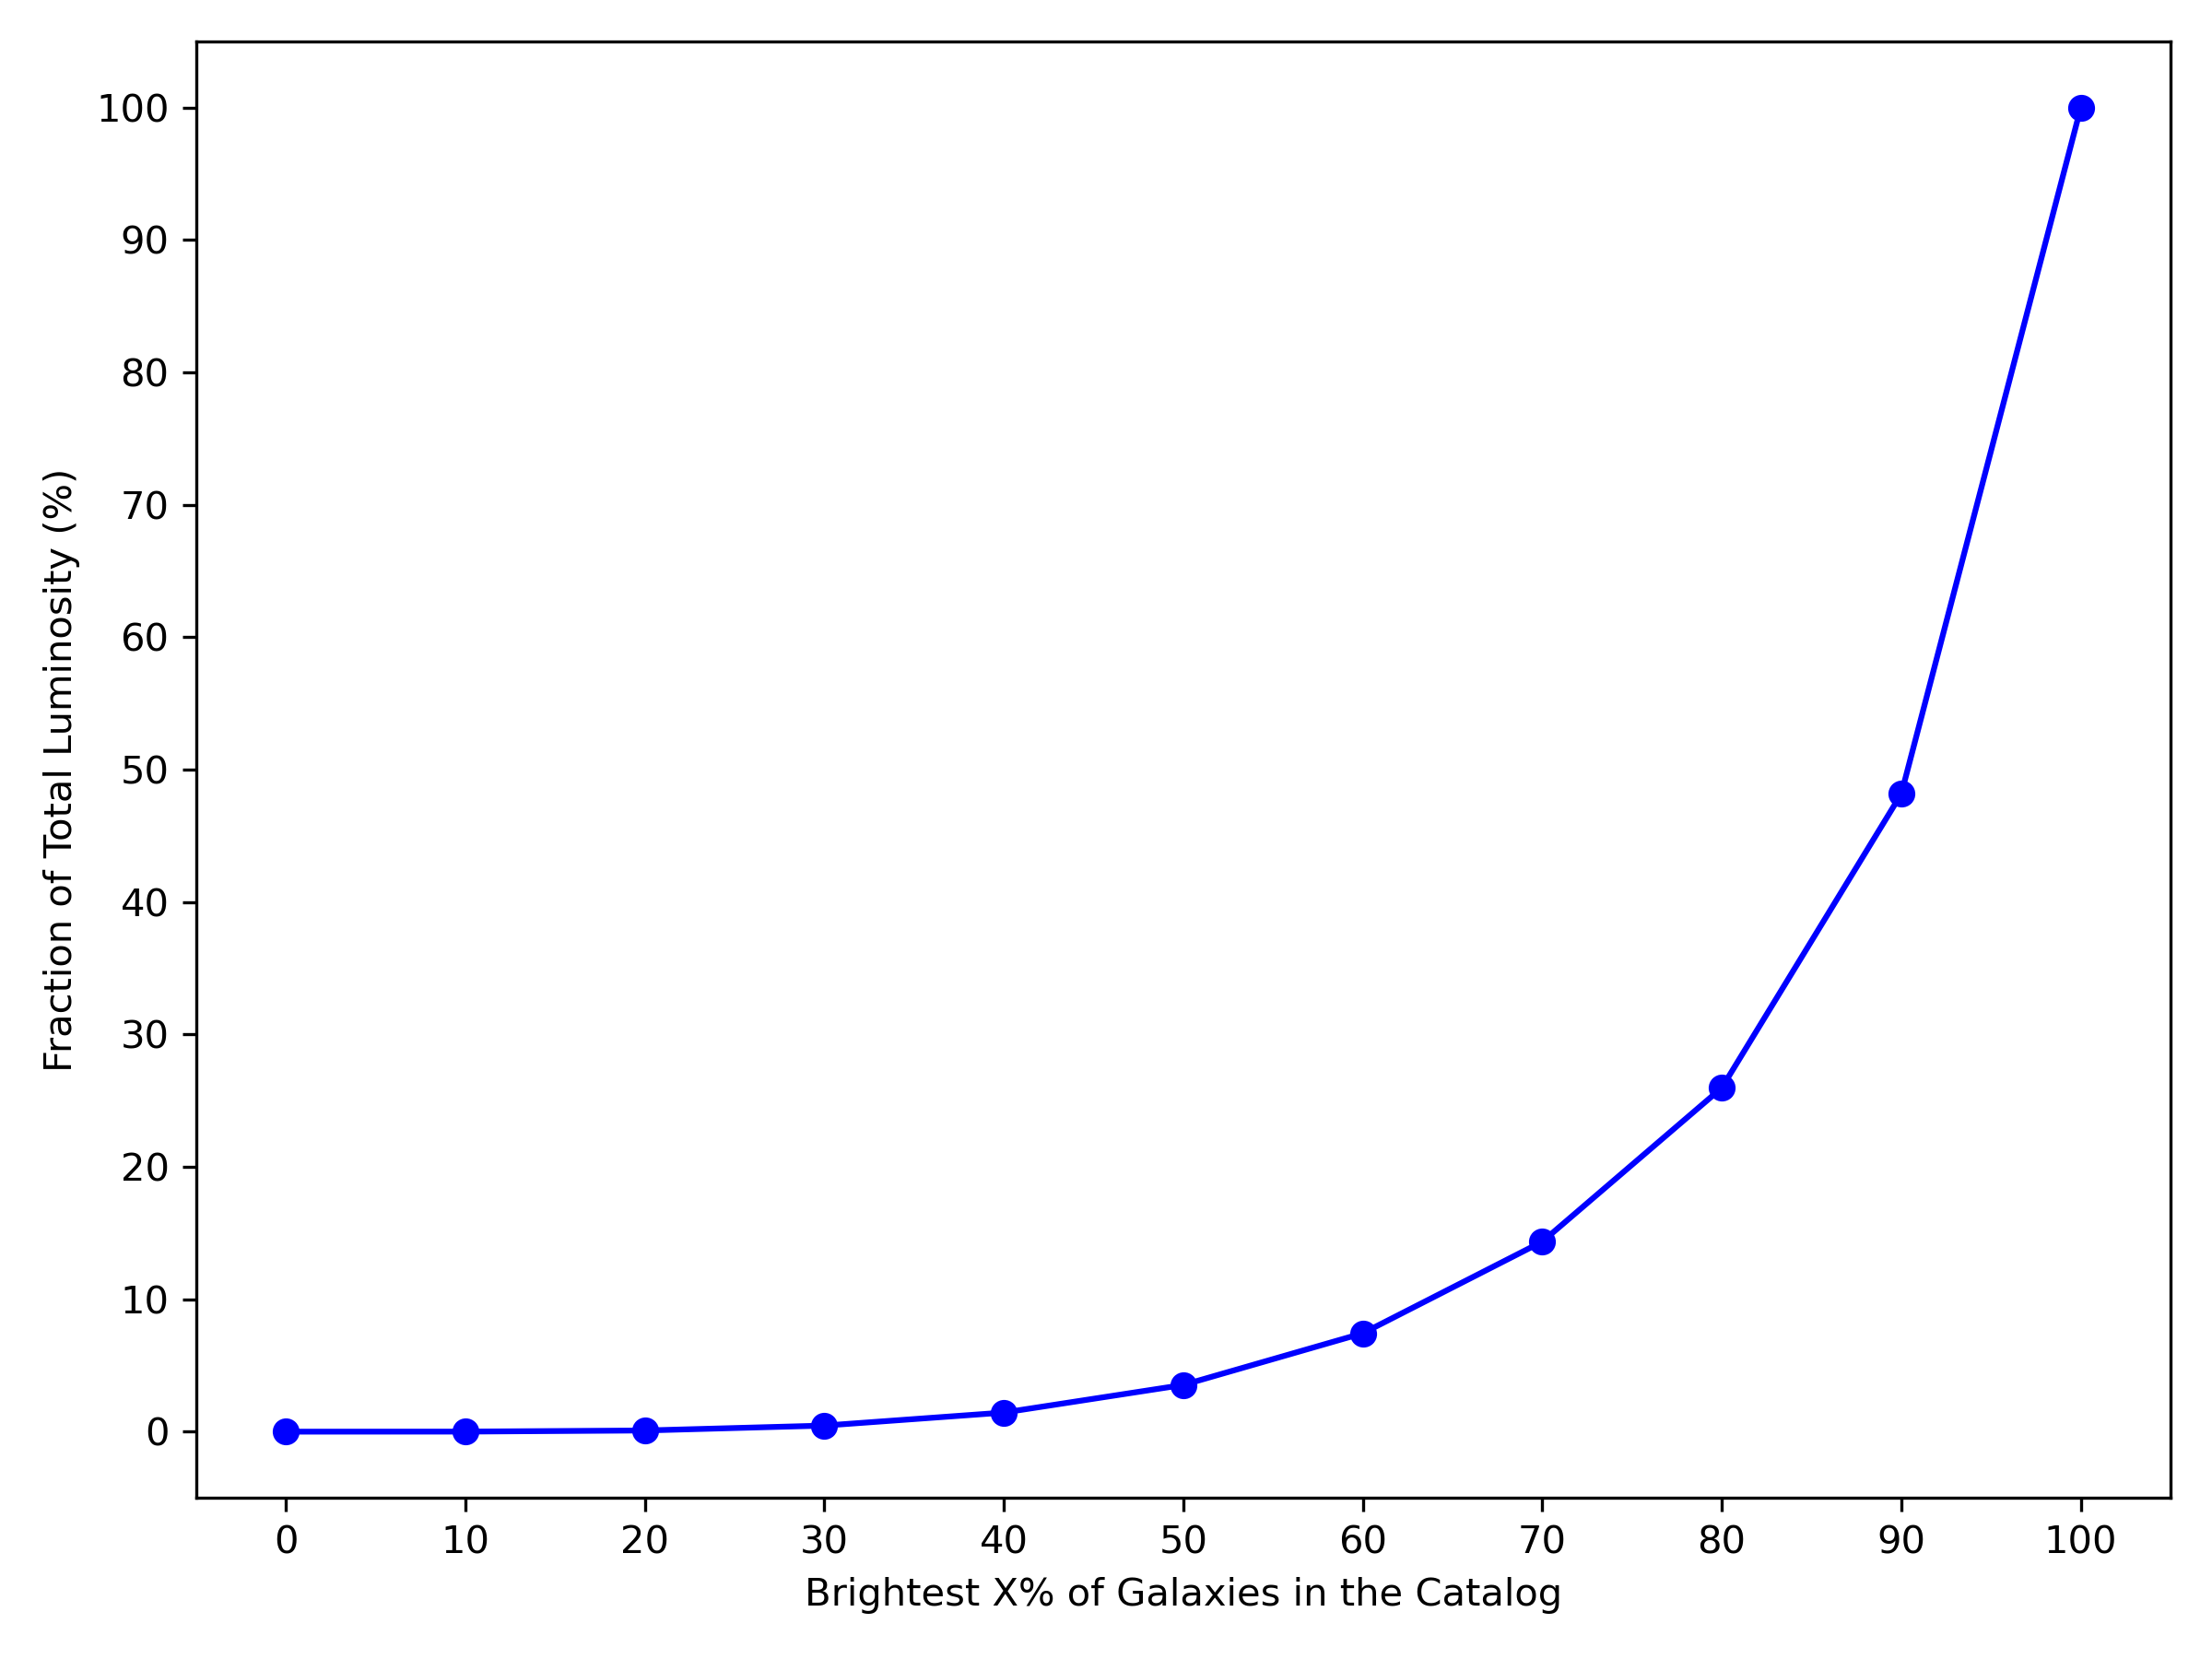
\includegraphics[width=0.7\textwidth]{figures/luminosity_fraction_vs_percentile_BUZZARD.png}
    \caption[\texttt{BUZZARD} luminosity retention.]{Fraction of total $K$-band luminosity as a function of the brightest $X\%$ of galaxies in the \texttt{BUZZARD} catalog. As in the real catalog, a steep decline occurs, driven by the large population of faint galaxies.\footnotemark}
    \label{fig:luminosity_buzzard}
\end{figure}
\footnotetext{This plot was generated using code partially adapted from scripts provided by Cezary Turski.}

This trend mirrors what was observed in the \texttt{GLADE+} analysis, reinforcing the idea that although brightness pruning excludes a large number of faint galaxies, the retained bright galaxies remain effective tracers of large-scale structure. This is further discussed in the next section. The plot also highlights that brightness-based selection inherently sacrifices a large fraction of integrated luminosity, an effect amplified when using an empirical catalog rather than applying a parametric model like the Schechter function. Nevertheless, these retained galaxies are the most cosmologically informative for our purposes.

\subsection{Tracing Large-Scale Structure with Luminous Galaxies}

\begin{figure}[h!]
    \centering
    \begin{subfigure}{0.5\textwidth}
        \centering
        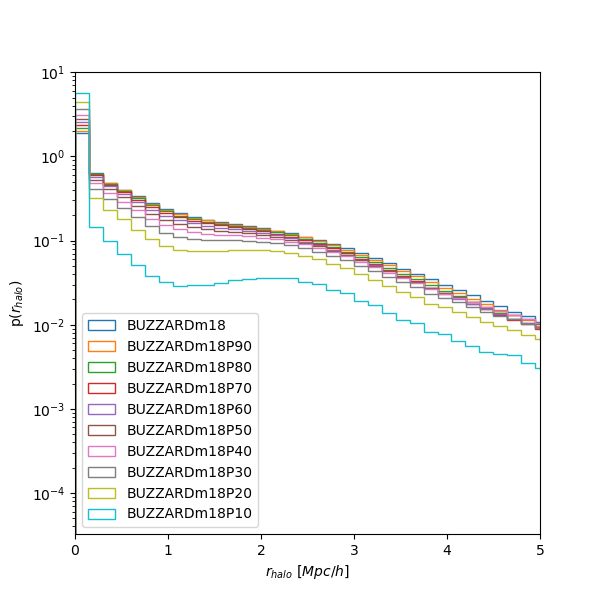
\includegraphics[width=\textwidth]{figures/rhalo_percentile.png}
    \end{subfigure}
    \hfill
    \begin{subfigure}{0.45\textwidth}
        \centering
        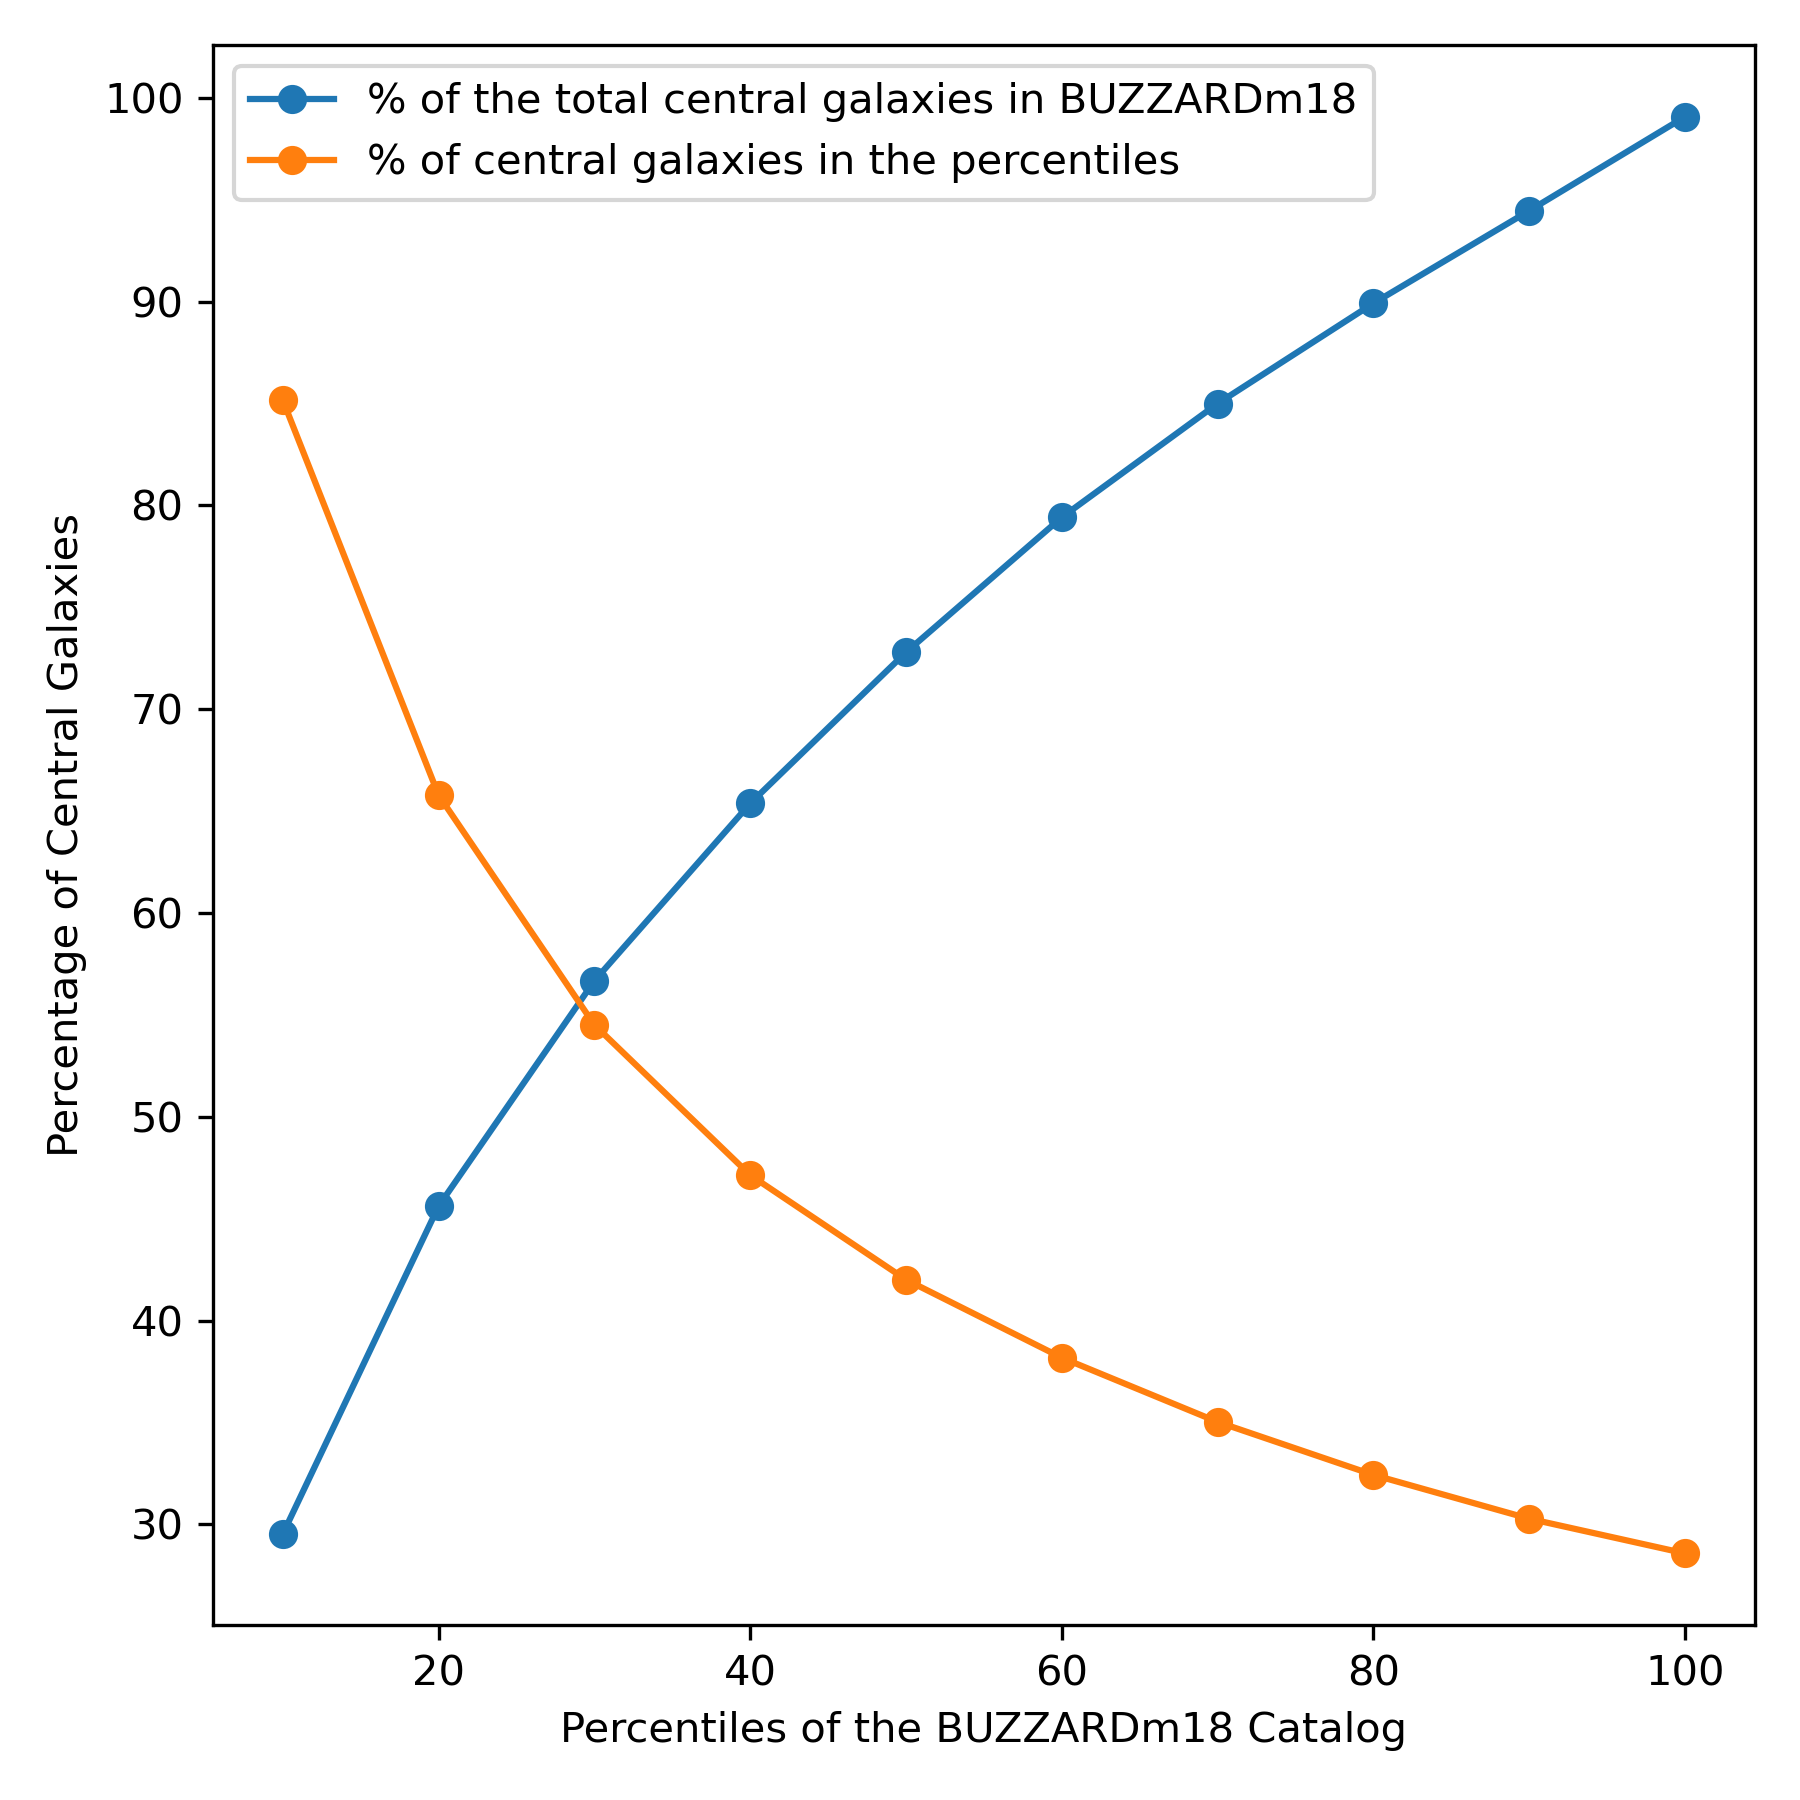
\includegraphics[width=\textwidth]{figures/central_gal.png}
    \end{subfigure}
    \caption[$r_{\mathrm{halo}}$ distribution and evolution for \texttt{BUZZARDm18} and its percentiles.]{\textbf{Left:} The distribution of the distance to the center of the nearest halo, $r_{\mathrm{halo}}$, for the \texttt{BUZZARDm18} catalog and its different percentiles, denoted \texttt{BUZZARdm18PXX}. \textbf{Right:} The evolution of the fraction of central galaxies in the \texttt{BUZZARDm18} catalog as a function of the brightness cut. The central galaxy fraction is defined as the ratio of the number of central galaxies, $r_{\mathrm{halo}} < 150~\mathrm{kpc}$, to the total number of galaxies in the catalog. The blue curve shows the remaining fraction of central galaxies when going from the \texttt{BUZZARDm18} catalog to the \texttt{BUZZARDm18PXX} catalogs, while the orange curve shows the fraction of central galaxies in the \texttt{BUZZARDm18PXX} catalogs.}
    \label{fig:MDC_rhalo}
\end{figure}

The \texttt{BUZZARD} mock catalog provides additional metadata for each galaxy, including its distance to the center of the nearest dark matter halo, denoted $r_{\mathrm{halo}}$. This information is crucial for assessing the spatial relationship between galaxies and the underlying matter distribution, and in particular, for identifying potential host galaxies for \ac{GW} events.

Figure~\ref{fig:MDC_rhalo} (left panel) shows the distribution of $r_{\mathrm{halo}}$ for the \texttt{BUZZARDm18} catalog and for various brightness-ranked subsets, denoted \texttt{BUZZARDm18PXX}. The distribution peaks at small radii ($r_{\mathrm{halo}} < 150$~kpc), corresponding to galaxies located at or near halo centers, with a long tail extending to larger radii. This indicates that a significant portion of the catalog consists of galaxies embedded in halos.

To quantify the effect of brightness cuts on the galaxy-halo relationship, we define \textit{central galaxies} as those with $r_{\mathrm{halo}} < 150$~kpc. The right panel of Figure~\ref{fig:MDC_rhalo} shows how the central galaxy fraction evolves across different brightness thresholds. The blue curve represents the retained fraction of central galaxies from the full \texttt{BUZZARDm18} catalog, while the orange curve shows the fraction of central galaxies within each \texttt{BUZZARDm18PXX} subset.

These plots reveal a clear trend: as we move to brighter percentiles, a large number of outer (non-central) galaxies are removed, while a substantial fraction of central galaxies are retained. In fact, the relative proportion of central galaxies increases with stricter pruning. This suggests that brightness cuts selectively preserve galaxies that are more likely to trace the centers of halos, thereby maintaining sensitivity to the large-scale structure despite an overall reduction in the catalog size.

\begin{table}
    \small
    \centering
    \caption[Central galaxy fraction for different $m_{\mathrm{thr}}$ for \texttt{BUZZARD}.]{Different apparent magnitude thresholds and their corresponding total number of galaxies and central galaxy fraction for the \texttt{BUZZARD} mock catalog.}
    \label{tab:MDC_catalogs}
    \begin{tabular}{c r c}
        \hline
        \textbf{$m_{\mathrm{thr}}$} & \textbf{Total Number of Galaxies} & \textbf{Central Galaxy Fraction} \\
        \hline
        $14$ & $41,018$ & $0.28$\\
        $16$ & $588,841$ & $0.29$ \\
        $18$ & $9,232,370$ & $0.29$ \\
        $20$ & $90,635,665$ & $0.13$ \\
        \hline
    \end{tabular}
\end{table}

Table~\ref{tab:MDC_catalogs} further supports this observation. It shows the central galaxy fraction for different apparent magnitude thresholds. Across $m_{\mathrm{thr}}$ = 14–18, the central galaxy fraction remains roughly constant near 30\%, but drops significantly for deeper thresholds (e.g., $m_{\mathrm{thr}}$ = 20) due to the increasing inclusion of dim, satellite, and field galaxies.

This behavior highlights an important point: although pruning the catalog to its brightest percentiles results in the loss of a large fraction of the total luminosity, this loss is largely due to the removal of numerous faint galaxies. The retained luminous galaxies, while fewer in number, are more likely to reside at halo centers and act as effective tracers of the matter distribution. Thus, the information most relevant for dark siren cosmology is preserved.

However, caution is warranted at the extreme end of pruning. For example, in the \texttt{BUZZARDm18P10} subset, while the majority of remaining galaxies are central, a significant number of central galaxies are also excluded. Given that only $\sim$30\% of galaxies in the full \texttt{BUZZARDm18} catalog are central, the best-case scenario implies that pruning below 30\% of the brightest galaxies inevitably leads to the loss of critical structure information and introduces potential bias.

This $\sim$30\% threshold appears robust across different magnitude cuts, as shown in Table~\ref{tab:MDC_catalogs}. For very deep catalogs ($m_{\mathrm{thr}} = 20$), the central galaxy fraction drops sharply, indicating a shift toward outer, dimmer galaxies that contribute less to the structure-tracing signal. Therefore, in our analysis with \texttt{GLADE+}, we should conservatively avoid cuts below this 30\% threshold to prevent loss of critical information.

Furthermore, Figure~\ref{fig:dist_gladep} illustrates that pruning primarily removes galaxies in the nearby Universe, while preserving structure at higher redshifts. This opens the possibility of constructing hybrid redshift priors, using a complete catalog for low-redshift volumes and brightness-ranked subsets for deeper regions. However, such an approach would require carefully stitching together two different \ac{LOS} redshift priors in a way that preserves smoothness and continuity, an effort that falls outside the scope of this thesis but represents an important direction for future work.

We should also be cautious about the fraction of central galaxies retained in the catalog, as excluding them disproportionately can bias the redshift distribution and thus affect cosmological inference. The \texttt{BUZZARD} catalog provides an ideal testbed to assess this impact in a controlled setting, where the true cosmology is known. Unfortunately, due to time constraints and technical challenges in processing and harmonizing the \texttt{BUZZARD} data, we were unable to conduct a full end-to-end bias quantification.

Nevertheless, the qualitative trends observed here and in partial mock runs strongly support the existence of a practical pruning floor around 30\% brightness, below which inference becomes unreliable. The end-to-end \ac{MDC} framework developed as part of this work is now operational, requiring only minor refinements to support such systematic studies in the future.

Identifying the optimal brightness cut and studying the bias it introduces in inferred $H_0$ values will be a natural and impactful extension of this work. It would allow us to rigorously assess the trade-off between catalog completeness and cosmological precision, and ensure that our pruning strategies do not introduce systematic errors into dark siren cosmology.